\documentclass{article}
\usepackage{amsmath, tikz, tkz-graph, tkz-berge}
\title{MATH 222 Assignment One}
\author{Oliver Tonnesen}
\date{September 17, 2018}
\begin{document}
\maketitle
\renewcommand{\thesubsection}{\thesection.\alph{subsection}}
\section{} % Section 1
Recall the following equation for a graph $G=(V,E)$:
\[\sum_{v\in{V}} {\deg(v)}=2|E|\]

We define $V_n$ to be the set $\{v|v\in{V},\deg(v)=n\}$.
\begin{align*}
	\sum_{v\in{V}} {\deg(v)} &= 250\\
	\sum_{v\in{V_4}} {\deg(v)} &= 44\\
	\sum_{v\in{V_5}} {\deg(v)} &= 125
\end{align*}
From this, we can see
\begin{align*}
	\sum_{v\in{V_3\cup{V_6}}} {\deg(v)} &= 250 - 44 - 125\\
	&= 81
\end{align*}
If we define $x$ to be the number of vertices of degree $3$, and $y$ to be the number of vertices of degree $6$, we can then derive the following equation:
\[81 = 3x+6y\]
We can see from our definition of $V_n$ that the following is true, since each vertex has exactly one degree
\[|V|=\sum_{i=0}^{n} {|V_i|}\]
So it follows that for some $V'\subseteq{V}$,
\[|V\setminus{V'}| = |V| - |V'|\]
So then, following similar logic as before, we can conclude that the number of vertices that are not of degree $4$ or degree $5$ is
\begin{align*}
	|V_3\cup{V_6}| &= |V| - |V_4| - |V_5|\\
	&= 56-11-25\\
	&= 20
\end{align*}
and so
\[20 = x+y\]
Now we can combine our two linear equations to solve for the number of vertices of degree 6, $y$
\begin{align*}
	20&=x+y\\
	x&=20-y\\\\
	81&=3x+6y\\
	81&=3(20-y)+6y\\
	81&=60-3y+6y\\
	21&=3y\\
	y&=7
\end{align*}
So the number of vertices of degree 6 is therefore 7.

\section{} % Section 2
\subsection{}
Place your knight on any space on the board and note the square's colour. Notice that each of the knight's possible moves fall on a space whose colour
is the opposite of that upon which the knight currently resides. Since this fact holds true for any space on the board, we have determined that the
knight can only travel from a black space to a white space and from a white space to a black space. More importantly, the knight can \underline{not}
travel from a black space to another black space or from a white space to another white space. So the graph representing the squares of the chessboard
can be partitioned into the set of vertices representing the black squares, $B$ and another set of vertices representing the white squares, $W$. Since the knight
we determined that the knight can not travel between squares of the same colour, $B$ and $W$ will form a bipartition.
\subsection{}
Each vertex has a degree of either 2, 3, 4, 6, or 8, depending on the proximity of the square it represents to the edge of the board.

\section{} % Section 3
\subsection{}
% https://graphtheoryinlatex.wordpress.com/2010/02/26/a-labeling-of-the-petersen-graph/
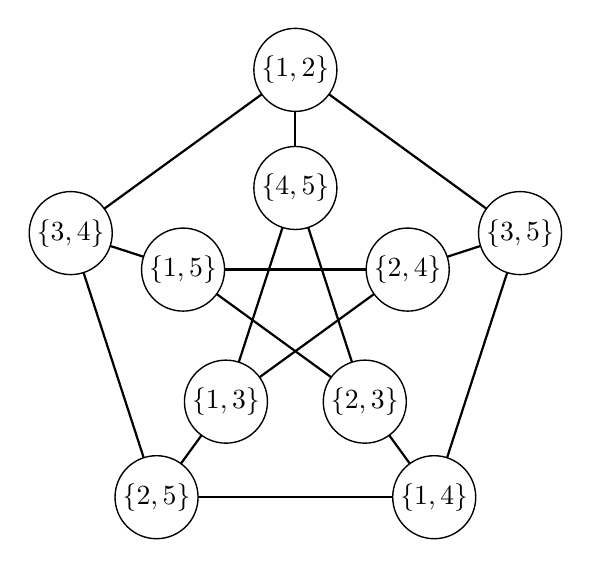
\begin{tikzpicture}[rotate=90]
		\newcommand{\aset}[2]{$\{#1,#2\}$}
		\GraphInit[vstyle=Normal]
		\SetVertexNoLabel
		\SetUpVertex[MinSize=30pt]
		\grPetersen[RA=3,RB=1.5]
		\AssignVertexLabel{a}{\aset{1}{2},\aset{3}{4},\aset{2}{5},\aset{1}{4},\aset{3}{5}}
		\AssignVertexLabel{b}{\aset{4}{5},\aset{1}{5},\aset{1}{3},\aset{2}{3},\aset{2}{4}}
\end{tikzpicture}

\subsection{}
Yes, see above.
\subsection{}
$G$ is a simple graph, so the edges will be left out of the trail for ease of viewing.
In the following trail, $\{1,2\},\{3,5\},\{1,4\}$ implicitly means $\{1,2\},\{1,2\}\{3,5\},\{3,5\},\{3,5\}\{1,4\},\{1,4\}$.
\[\{1,2\},\{3,5\},\{1,4\},\{2,5\},\{3,4\},\{1,2\},\{4,5\},\{2,3\},\{1,5\},\{2,4\},\{1,3\},\{4,5\}\]


\section{} % Section 4
\subsection{}
Each vertex in $G$ has degree 3, so it is the middle vertex in $\binom{3}{2}$ distinct copies of $P_3$.
$G$ has $10$ vertices, and so the number of copies of $P_3$ contained in $G$ is equal to
\[10\binom{3}{2}=30\]
\subsection{}
Take some vertex $v\in{V}$. $v$ is the first vertex in the path $P_4$ for $3\cdot2\cdot2=12$ paths. Likewise, $v$ is the \textit{last} vertex
in the path for some $12$ other paths. So the sum of the number of paths for which each $v\in{V}$ is the first vertex counts twice the number
of copies of $P_4$ in $G$.
\[\dfrac{10\cdot12}{2}=60\]
\subsection{}
$C_5$ is a cycle on $5$ vertices, so if all the cycles beginning at each vertex $v\in{V}$ are counted, each cycle will be counted $5$ times, once
for each vertex it consists of. Any one vertex $v\in{V}$ is a part of $4$ distinct copies of $C_5$, so the total number of copies of $C_5$ contained in
$G$ is equal to
\[\dfrac{10\cdot4}{5}=20\]

\section{} % Section 5
\subsection{}
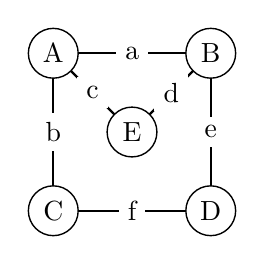
\begin{tikzpicture}
	\Vertex{A}
	\Vertex[x=2,y=0]{B}
	\Vertex[x=0,y=-2]{C}
	\Vertex[x=2,y=-2]{D}
	\Vertex[x=1,y=-1]{E}

	\Edge[label={a}](A)(B)
	\Edge[label={b}](A)(C)
	\Edge[label={c}](A)(E)
	\Edge[label={d}](B)(E)
	\Edge[label={e}](B)(D)
	\Edge[label={f}](C)(D)
\end{tikzpicture}
\newline
Hamiltonian Cycle:
\[A,c,E,d,B,e,D,f,C,b,A\]
Eulerian Circuit:
A has degree 3, and so does not satisfy the property of Eulerian circuits that each vertex has an even degree. Thus this graph can not have an Eulerian circuit.
\subsection{}
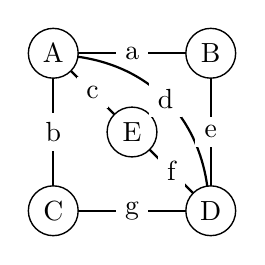
\begin{tikzpicture}
	\Vertex{A}
	\Vertex[x=2,y=0]{B}
	\Vertex[x=0,y=-2]{C}
	\Vertex[x=2,y=-2]{D}
	\Vertex[x=1,y=-1]{E}

	\Edge[label={a}](A)(B)
	\Edge[label={b}](A)(C)
	\Edge[label={c}](A)(E)
	\tikzset{EdgeStyle/.style = {-,bend left=37}}
	\Edge[label={d}](A)(D)
	\tikzset{EdgeStyle/.style = {-}}
	\Edge[label={e}](B)(D)
	\Edge[label={f}](E)(D)
	\Edge[label={g}](C)(D)
\end{tikzpicture}
\newline
Hamiltonian Cycle: Every vertex in a cycle must have a degree of exactly 2. Since each of $B$, $C$, and $E$ is only adjacent to $A$ and $D$,
all three of them must have an edge connecting to both $A$ and $D$. Thus each of $A$ and $D$ must have a degree of at least 3 and so there can
exist no cycle in this graph, Hamiltonian or otherwise.\\
Eulerian Circuit:
\[A,a,B,e,D,g,C,b,A,c,E,f,D,d,A\]
\subsection{}
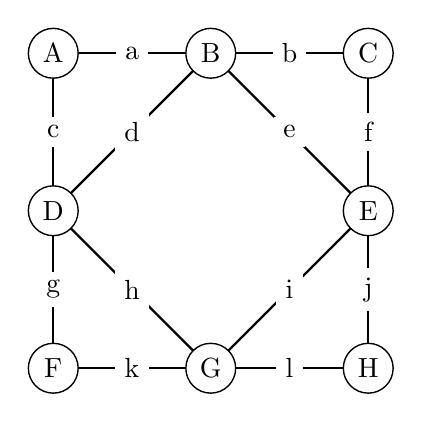
\begin{tikzpicture}
	\Vertex{A}
	\Vertex[x=2,y=0]{B}
	\Vertex[x=4,y=0]{C}
	\Vertex[x=0,y=-2]{D}
	\Vertex[x=4,y=-2]{E}
	\Vertex[x=0,y=-4]{F}
	\Vertex[x=2,y=-4]{G}
	\Vertex[x=4,y=-4]{H}

	\Edge[label={a}](A)(B)
	\Edge[label={b}](B)(C)
	\Edge[label={c}](A)(D)
	\Edge[label={d}](B)(D)
	\Edge[label={e}](B)(E)
	\Edge[label={f}](C)(E)
	\Edge[label={g}](D)(F)
	\Edge[label={h}](D)(G)
	\Edge[label={i}](E)(G)
	\Edge[label={j}](E)(H)
	\Edge[label={k}](F)(G)
	\Edge[label={l}](G)(H)
\end{tikzpicture}
\newline
Hamilton Cycle:
\[A,a,B,b,C,f,E,j,H,l,G,k,F,g,D,c,A\]
Euclidean Circuit:
\[A,a,B,b,C,f,E,j,H,l,G,k,F,g,D,d,B,e,E,i,G,h,D,c,A\]

\section{} % Section 6
Consider some disconnected graph $G=(V,E)$. By definition, there must exist some $S=\{v_1,v_2,\ldots,v_n\}\subseteq{V}$ such that for any two
vertices $u_1,u_2\in{S}$ there exists no path $u_{1}u_{2}\in{E}$.
Now consider the $n$ components of $G$: $C_1,C_2,\ldots,C_{n}$. Every vertex in $C_m$ is reachable from $v_m$, and is \textit{not}
reachable from any vertex $v_l\in{S}, l\neq{m}$. This means that in $\overline{G}$, every vertex in ${C_n}$ will have a path to every
vertex in every other component. Most importantly, each vertex in $C_n$ will have a path to every vertex $u\in{S}$, $u\neq{v_n}$.
This also means that in $\overline{G}$, $S$ will represent the vertices of a complete subgraph on $n$ vertices, $K_n$. Thus, since every vertex in
$S$ is connected and every other vertex is connected to at least one vertex in $S$, there must exist a path between any two vertices in $V$, and so
$\overline{G}$ must be connected.

\section{Bonus} % Section 7
Let $P=v_0v_1v_2\ldots{v_n}$ be the longest path in $G$. $v_0$ has at least $k$ neighbors. If $v_0$ has a neighbor that is not in $P$, then $P$ can be
extended and is not the longest path in $G$. Thus each of $v_0$'s neighbors are in $P$. Let $v_0$'s neighbor that comes latest in $P$ (from $v_0$ to $v_n$)
be $v_l$. Since $v_0$ has at least $k$ neighbors in $P$, that which comes the latest must be at least the ${(k+1)}^{th}$ vertex in $P$. Thus the length of
the path $v_0v_1v_2\ldots{v_l}$ is at least $k+1$. Since $v_l$ is, by definition, a neighbor of $v_0$, there must exist a walk $v_0v_1v_2\ldots{v_l}v_0$:
a cycle on at least $k+1$ vertices.

\end{document}
